%%%%%% CMB-S4 Simulations and Data Analysis Chapter, Component Separation Section  %%%%%%%%%%%%%%%%

\section{Component Separation}

\textbf{ Authors: Mark Ashdown, Jonathan Aumont, Carlo Baccicalupi, Josquin Errard, Maude Le Jeune}

Key challenges:
\begin{itemize}
\item validation - are we using the right algorithms for the (as yet unknown) real foregrounds
\item verification - are these algorithms right given our (as yet flawed) simulations
\end{itemize}

\begin{figure*}[htbp]
\centering
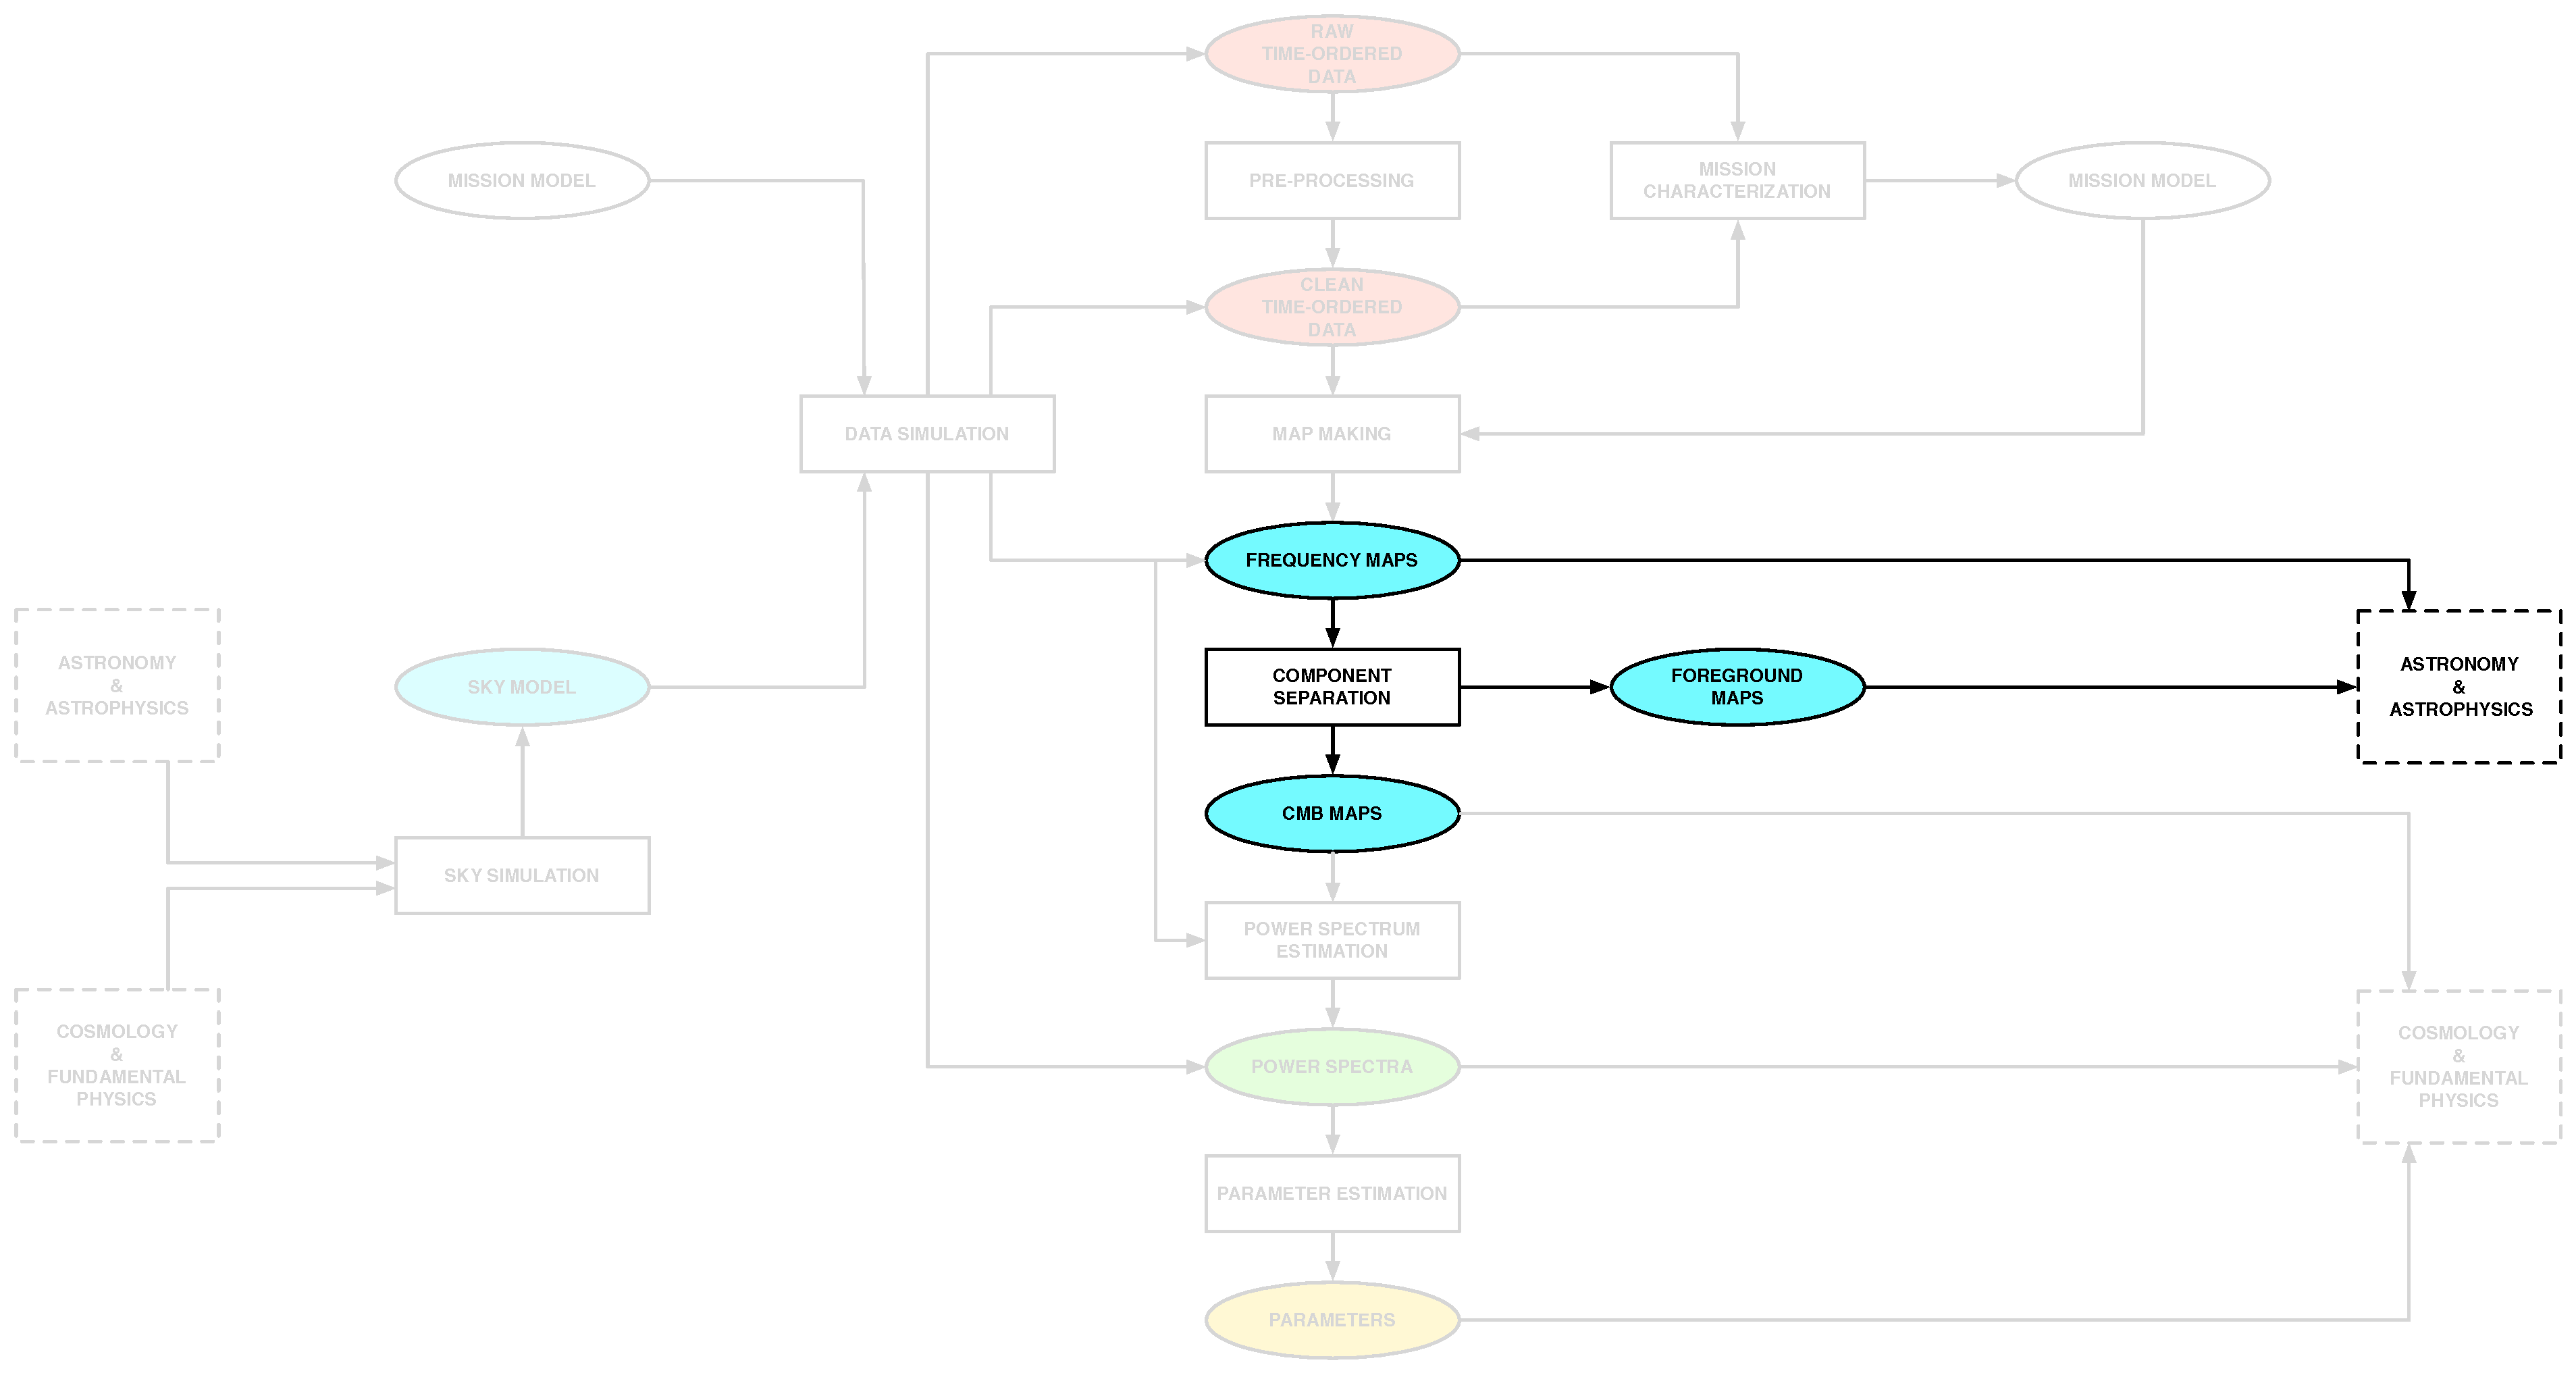
\includegraphics[width=1\textwidth]{Analysis/cs}
\caption{The component separation subset of the CMB simulation and data analysis pipeline}
\label{default}
\end{figure*}

This section discusses the algorithms and methods disentangling sky emissions from multi-frequency maps. 
We first present the motivations and the general ideas of existing methods. 
We then give the specificities of parametric and blind methods. 
Finally, we summarize several questions which might be answered by follow-up studies.

\subsection{Introduction}

\begin{figure*}[htbp]
\centering
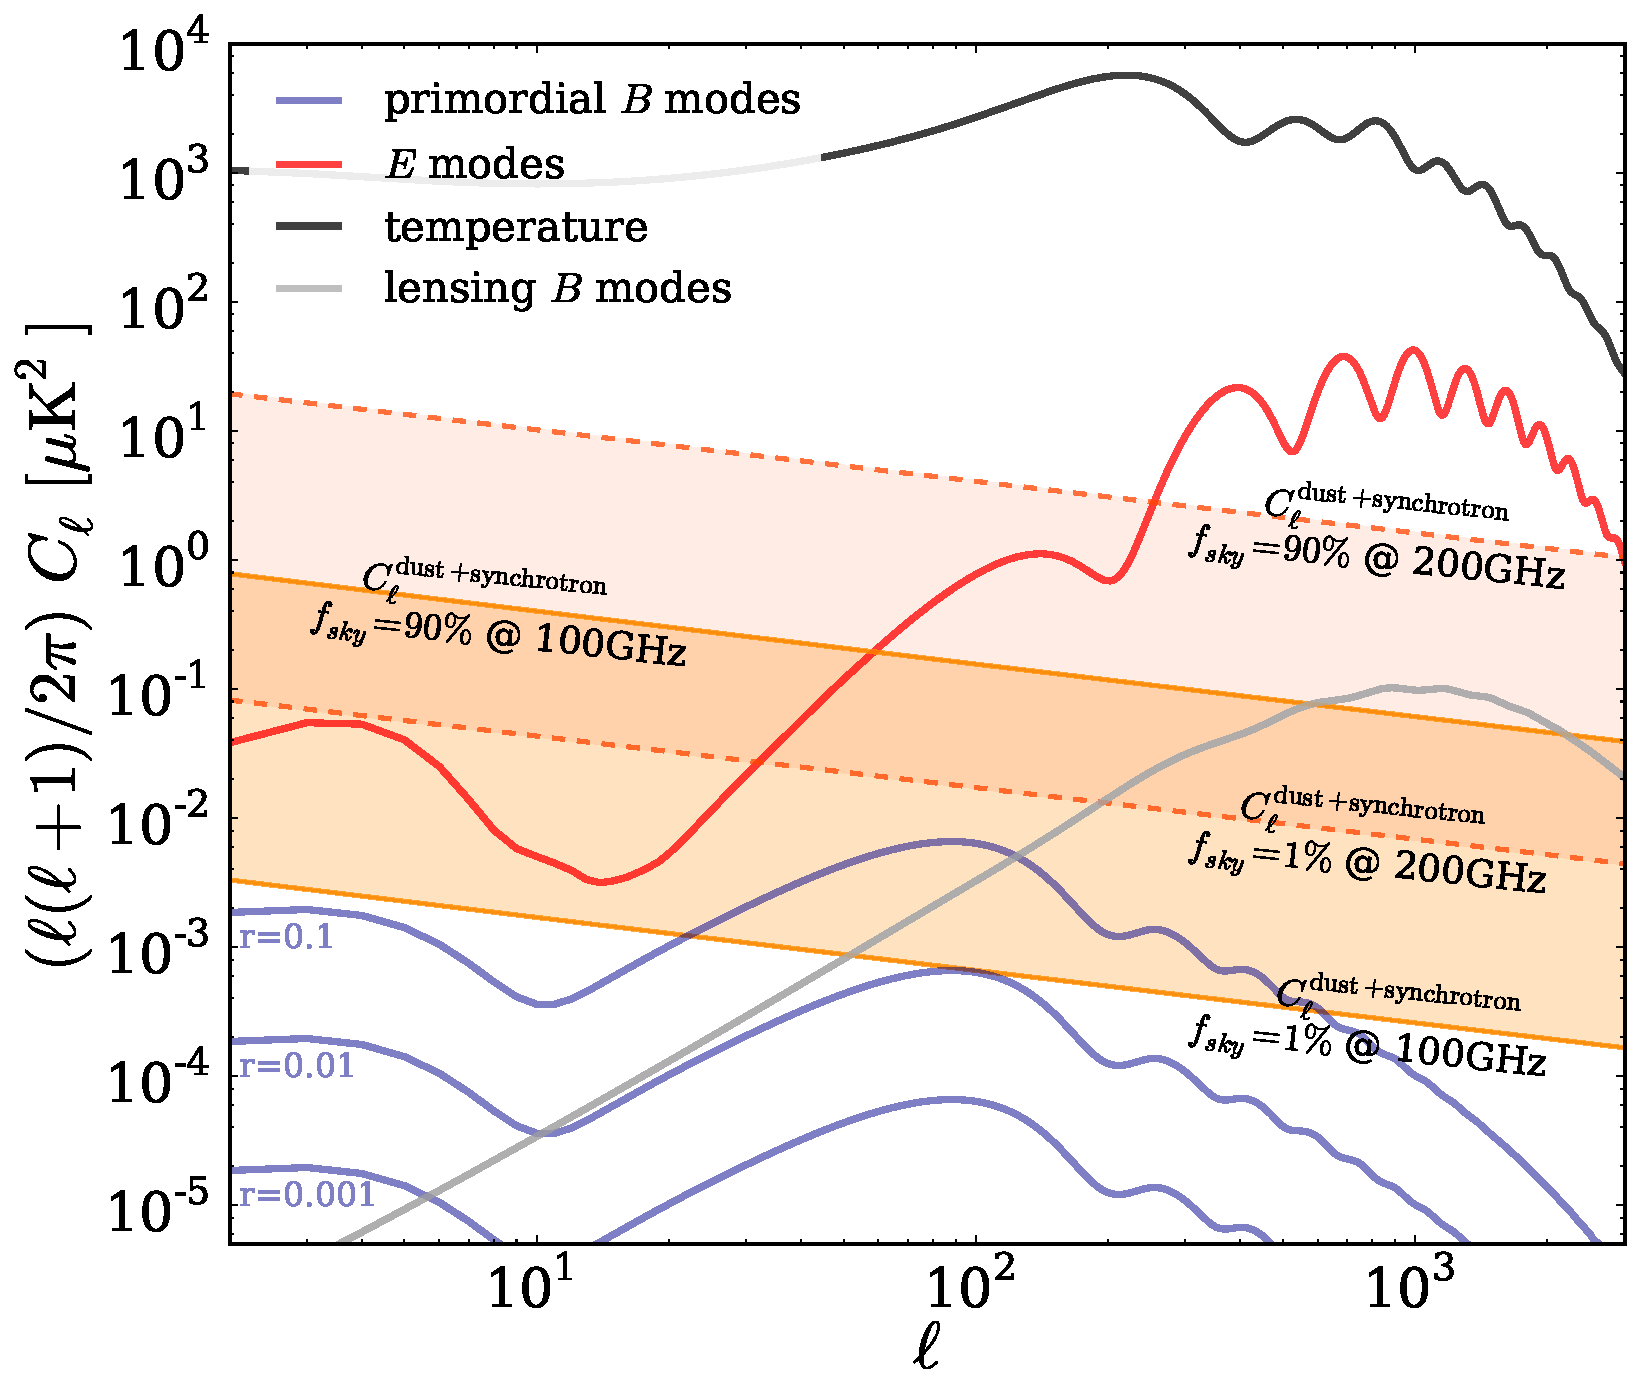
\includegraphics[width=0.5\textwidth]{Analysis/Power_Spectrum_figure_showing_foregrounds.pdf}
\caption{Angular power spectra showing primordial $B$ modes, lensing $B$ modes, total intensity, and $E$ modes, as well as the total contribution of polarized $B$-mode foregrounds (dust plus synchrotron), expected on the cleanest $1-90\%$ of the sky, at $100$ and $200\;$GHz. Note that, as these results are derived from Planck's Galactic masks and are not therefore optimized for high-resolution, ground-based instruments, there is potential for discovery of small patches of sky (e.g., $f_{\mathrm sky} \leq 5\%$) cleaner than those indicated here. From~\cite{}.}
\label{default}
\end{figure*}


\subsubsection{Motivations}

S4 science goals are $r$ and neutrino mass
\begin{itemize}
	\item component separation is obviously a necessary step to go beyond current constraints on e.g. primordial B-modes, cf. e.g. Fig.  of Errard et al (2015) --- foregrounds residuals coudl be expected to be dominant on largest scales?
	\item for neutrino mass, I suppose $C_\ell^{dd}$ has the best lever-arm, and we should evaluate the impact of foregrounds on the 4-point function (E-B estimators I suppose). NB: Planck lensing 2015 is based on SMICA map. Yet, the use of multiple-resolution maps degrades the final resolution of the component separated maps compared to a simple quadratic combination of beams weighted by their corresponding sensitivity. This might impact constraints on the lensing BB peak.
\end{itemize}

%%%%%%%%%%%%%%%%%%%%%%
\subsubsection{Definition of component separation}
The general data modeling assumes that, for each sky pixel $p$, one has
\begin{eqnarray}
	\centering	
		d_p = \mathbf{A}s_p + n_p
	\label{eq:comp_sep_data_modeling}
\end{eqnarray}
where the vector $d$ contains the measured amplitude from each frequency map, $\mathbf{A}$ is the so-called mixing matrix, $s_p$ is a vector containing the unknown CMB and foregrounds amplitude and $n_p$ is vector containing the noise corresponding to each frequency band.

Given this modeling, the component separation aims at inverting Eq.~\ref{eq:comp_sep_data_modeling}, to estimate the foregrounds-distangled CMB signal encapsulated in $s_p$. 
The general solution to Eq.~\ref{eq:comp_sep_data_modeling} would be given by
\begin{eqnarray}
	\centering
		\tilde{s}_p = \mathbf{W}d_p
	\label{eq:sp_solution}
\end{eqnarray}
where $\mathbf{W}\equiv  \left( \mathbf{A}^T\mathbf{N}^{-1}\mathbf{A} \right)^{-1}\mathbf{A}^T\mathbf{N}^{-1}$ gives an unbiased estimate of the sky.

The component separation methods would generally
\begin{itemize}
	\item include any data processing that characterizes and exploit correlations between multi-frequencies observations,
	\item put external constraints and physical modeling
	\item and it would aim at distinguishing between different physical sources of emission.
	%NB For a given method, one would think that there should be a validation step (do the tools work on reasonable sky models?) and a verification step (are the sky models consistent with reality?). The second step is obviously the most difficult to answer.
\end{itemize}

$\rightarrow$ feedback from Planck component separation as well as the early CMB cleaning achieved in the BKP measurements + Stivoli et al (2010) + Fantaye et al (2011+2012) + Errard et al (2011+2012+2015).

%%%%%%%%%%%%%%%%%%%%%%
\subsection{Description of methods}
The overall idea of component separation boils down to two steps:
\begin{itemize}
	\item estimation of the mixing matrix, $\mathbf{A}$;
	\item inversion of Eq.~\ref{eq:comp_sep_data_modeling} to recover an estimate of the sky signal, $s_p$.
\end{itemize}
The second step being is rather general to any component separation cf. ..., whereas the first step can be performed in various ways:
\begin{itemize}
	\item \textbf{Parametric} -- it assumes that the mixing matrix, used in Eq.~\ref{eq:comp_sep_data_modeling}, can be parametrized $\mathbf{A} = \mathbf{A}(\beta)$. The functional form of $\mathbf{A}$ being fixed, the estimation of the mixing matrix is therefore equivalent to an estimation of the parameters $\beta$. This is usually down by maximizing the following likelihood cf.....
	\begin{eqnarray}
		\centering
			-2\log \mathcal{L}(\beta) = - \sum_p \left( \mathbf{A}^T\mathbf{N}^{-1} d\right)^T\left( \mathbf{A}^T\mathbf{N}^{-1} \mathbf{A}\right)^{-1}\left( \mathbf{A}^T\mathbf{N}^{-1} d\right)
	\end{eqnarray}
	\item \textbf{Blind} (Maude)
	\item \textbf{Discussion regarding the domain of application (harmonic, pixel, wavelet,etc.)} -- 
\end{itemize}

$\rightarrow$ Parametric fitting vs. ILC, spatial domain versus non-spatial, that makes a basis of 4 algorithms. Although it was never quantified, the independence of those and very different hypotheses represent an opportunity for cross-checking and robustness.

%%%%%%%%%%%%%%%%%%%%%%
\subsection{Questions to be addressed during follow-up studies}
\begin{itemize}
	\item pros/cons for E/B vs Q/U
	\item pros/cons for multi-sites
	\item pros/cons for having various resolutions
	\item atmosphere residuals and dust in maps could scale similarly with frequency...
	\item we could outline a roadmap, i.e. the application and learning phase to SIV made by the various sub-orbitals which are going on-line now or soon with the usual 95, 150, 220. That would need to be investigated very accurately as it would represent a most important step for component separation
towards SIV.
\end{itemize}





%\bibliography{cmbs4}

%%
%% Populate the .bib file with entries from SPIRES Bibtex (preferred)
%% or ADS Bibtex (if no SPIRES entry).
%%  SPIRES will also supply the CITATION line information; please include it.
%%


